\documentclass{beamer}
\usepackage[utf8]{inputenc}
\usepackage[]{amsmath}
\usepackage{graphicx}
\usepackage{physics}
\usepackage{subcaption} % package pour faire des subfigures
\usepackage{multirow} % package pour multirow/multicolumn
\usepackage{booktabs} % package pour top/mid/bottom rule
\usepackage{tcolorbox} % toujours plus de boites
%\usepackage[backend=biber]{biblatex}
%
%
%\addbibresource{Biblio_dbl_quantum.bib}

%\bibliographystyle{stylename}
%\bibliography{Biblio_dbl_quantum}

\title{Dipolar interactions in dense ensembles of Nitrogen-Vacancy centers}
\author{Clément Pellet-Mary, Maxime Perdriat, Gabriel Hétet}
\date{Nano-optics group}

\mode<presentation> {\usetheme{Rochester}}

\begin{document}
\begin{frame}
\maketitle
\begin{center}
\includegraphics[width=\textwidth,height=0.3\textheight,keepaspectratio]{logos}
\end{center}
\end{frame}
%\begin{frame}{Outline}
%\tableofcontents
%\end{frame}
%\section{Physics of the NV center}
\begin{frame}{Preamble : the NV center}
\centering
\includegraphics[width=\textwidth,height=0.9\textheight,keepaspectratio]{Slide  NV properties}
\end{frame}

\begin{frame}{Preamble : the 4 classes of NV centers}
\centering
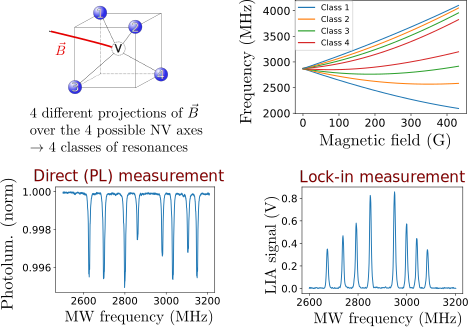
\includegraphics[width=\textwidth,height=0.9\textheight,keepaspectratio]{slide ODMR 4 classes}
\end{frame}

\begin{frame}{Subject of this presentation}
\centering
\includegraphics[width=\textwidth,height=0.9\textheight,keepaspectratio]{slide_presentation_sujet}
\end{frame}

\begin{frame}{Outline}
\tableofcontents
\end{frame}

\section{Cross-relaxation with NV centers}
\begin{frame}{Principle of cross-relaxation with NV centers}
\centering
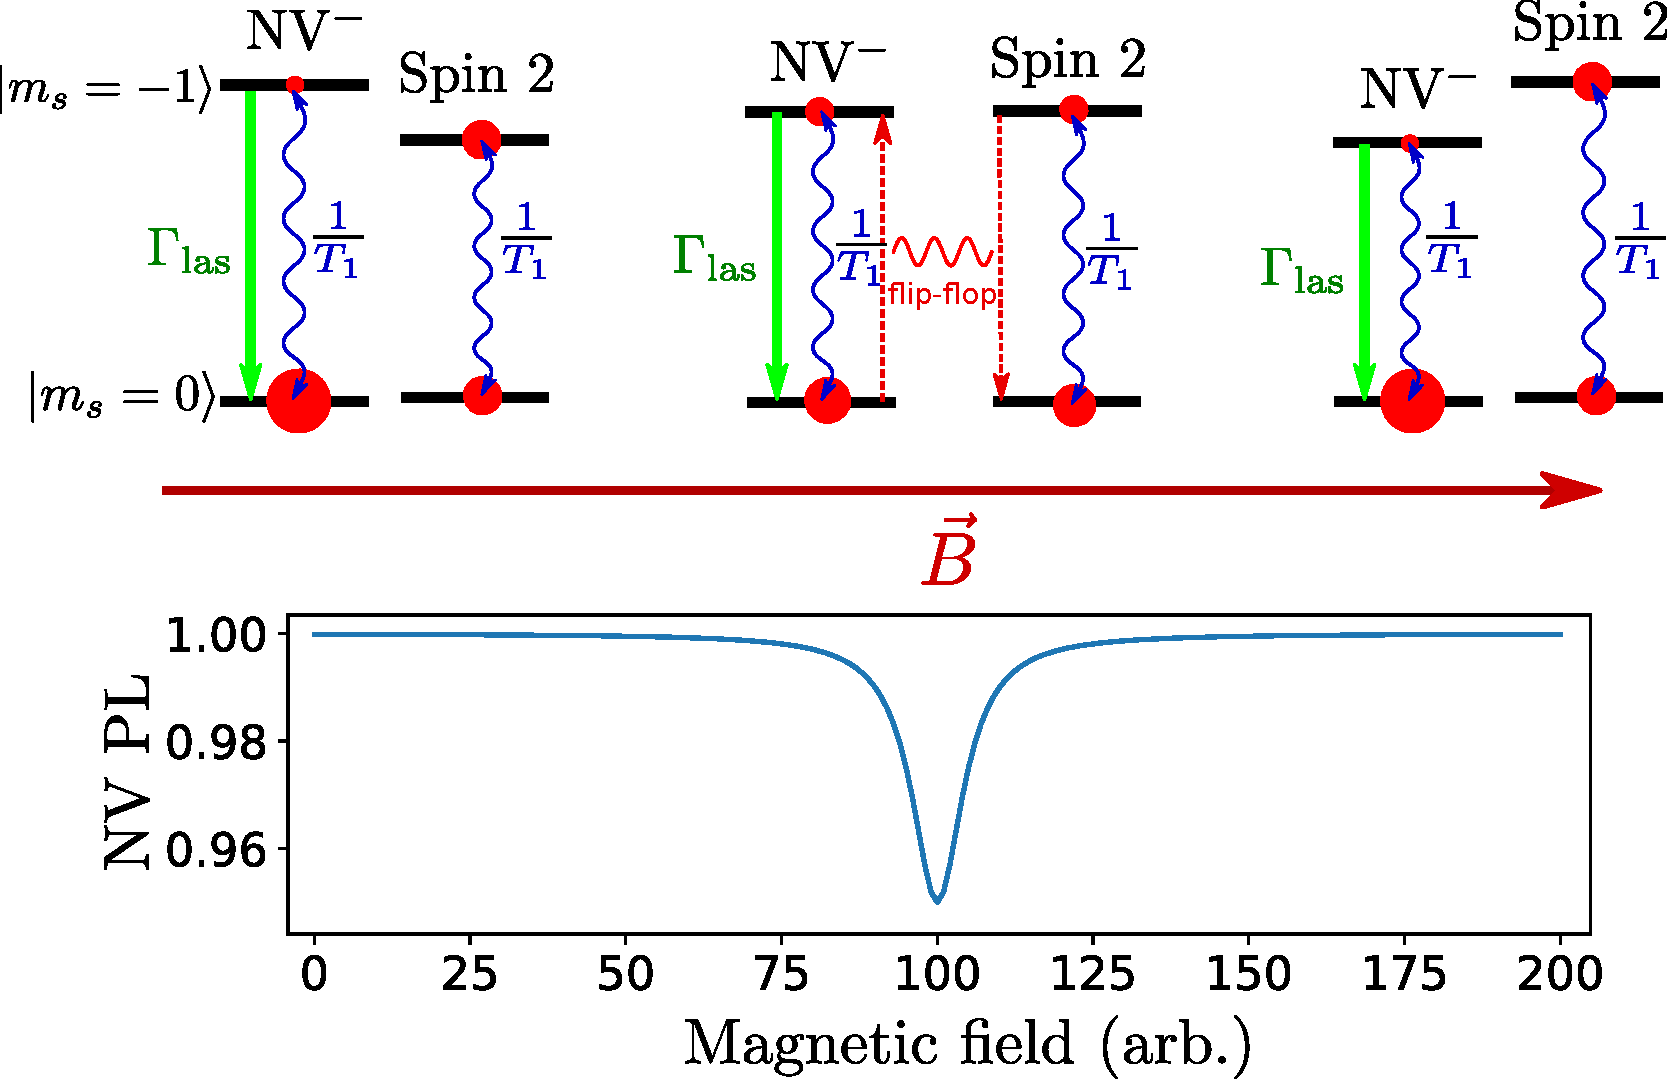
\includegraphics[width=\textwidth,height=0.8\textheight,keepaspectratio]{Slide_CR_presentation}
\end{frame}

\begin{frame}{Example: Cross-relaxation between NV centers and VH$^-$}
\centering
\includegraphics[width=\textwidth,height=0.9\textheight,keepaspectratio]{Slide_CR_VH}
\end{frame}

\begin{frame}{Cross-relaxation between NV centers and NV centers}
\centering
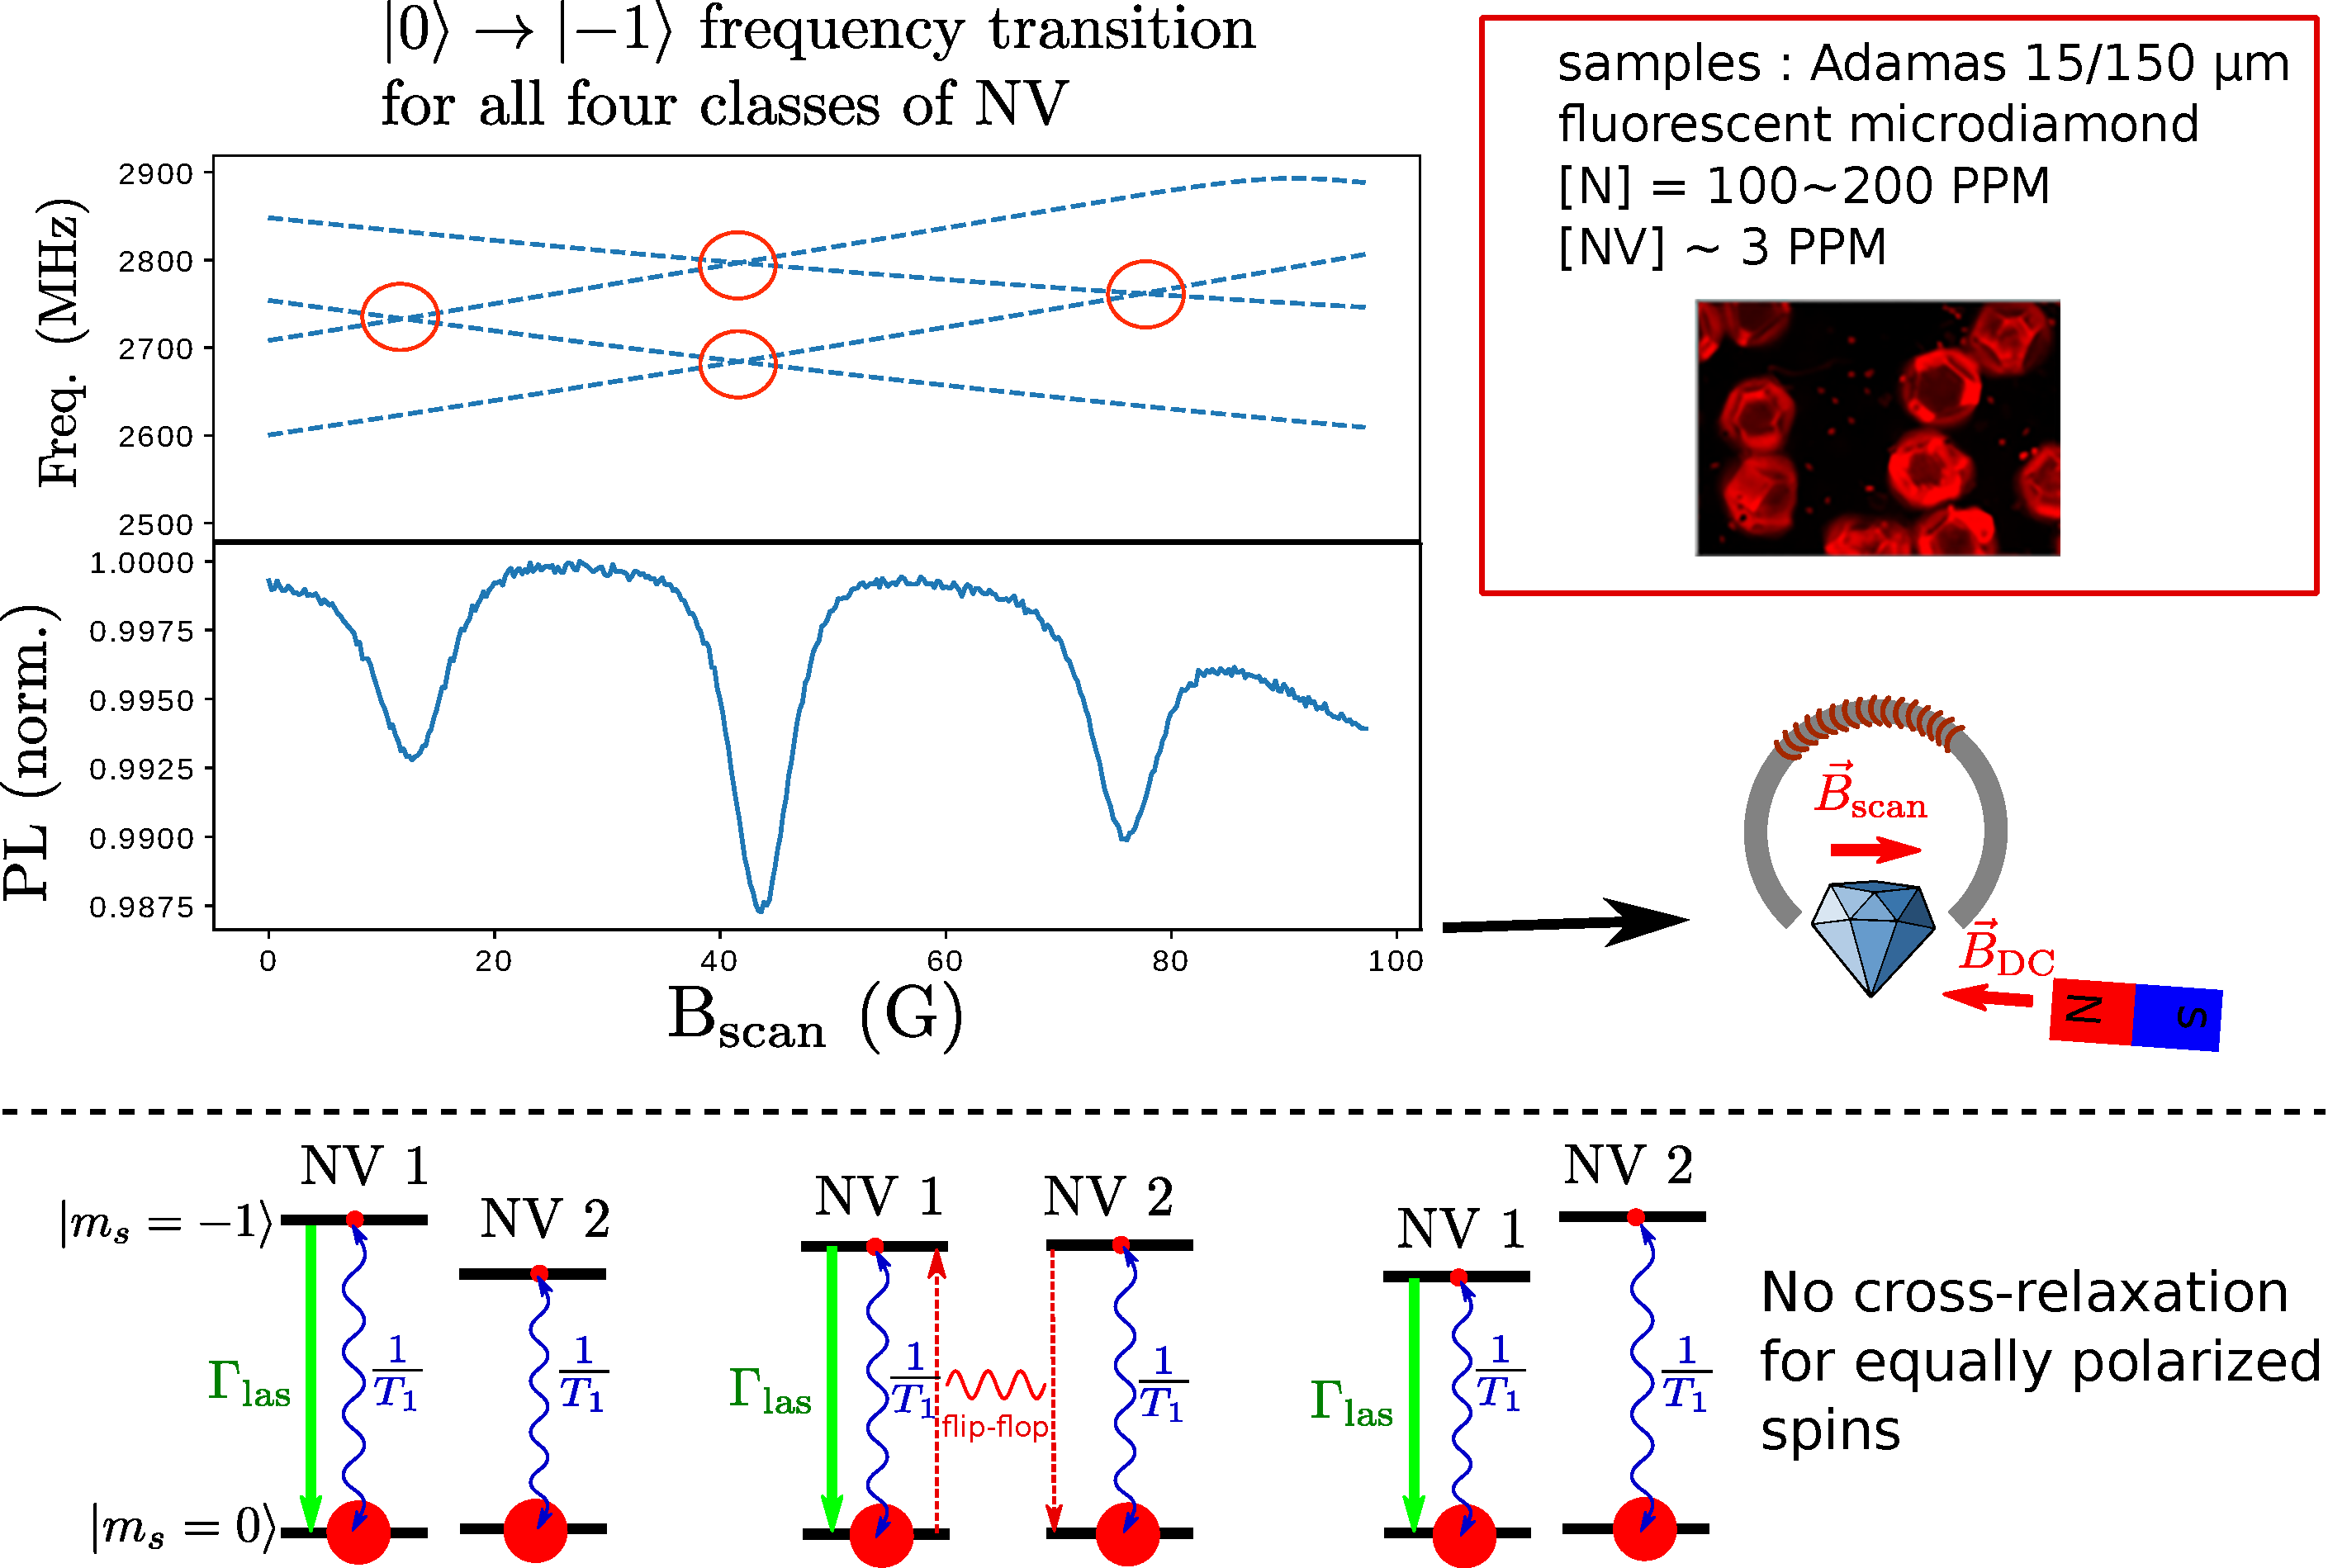
\includegraphics[width=\textwidth,height=0.9\textheight,keepaspectratio]{Slide_CR_adamas}
\end{frame}
\section{The NV-fluctuator model and experimental verification}

\begin{frame}{Presentation of the fluctuator model}
\centering
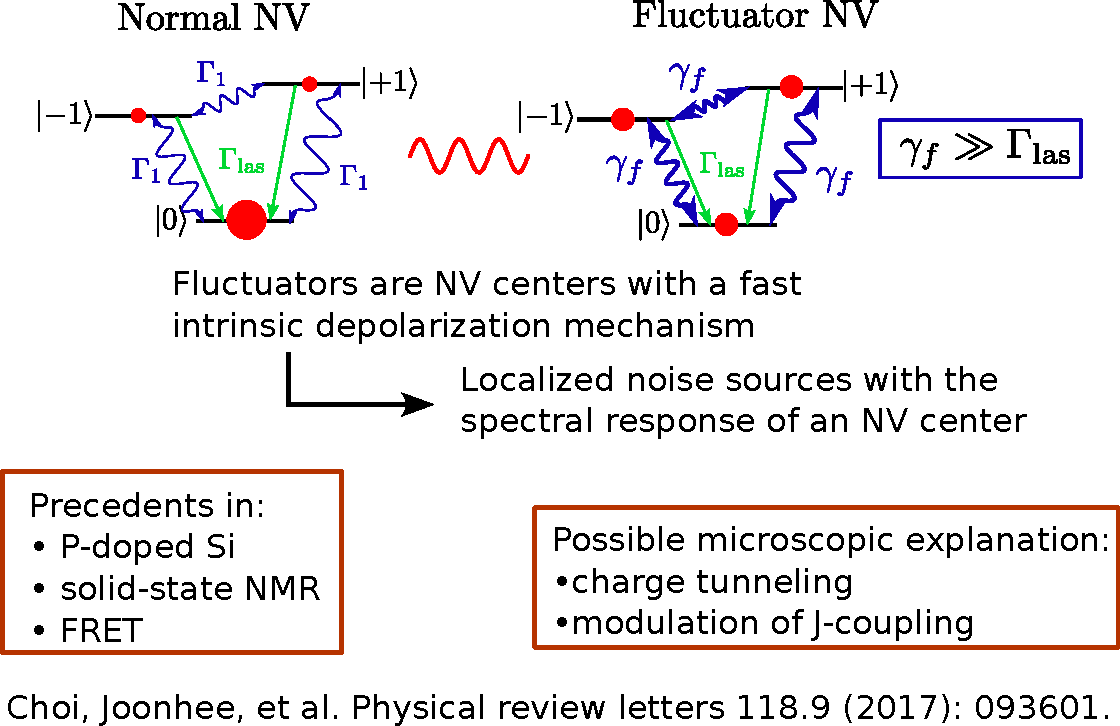
\includegraphics[width=\textwidth,height=0.8\textheight,keepaspectratio]{Slide_fluct_intro}
\end{frame}

\begin{frame}{Predictions of the fluctuator model}
\begin{itemize}
\item $\Gamma_1$ increases when classes overlap spectrally (increase in the resonant fluctuator density).
\item The dipole induced depolarization has a stretched exponential profile:
$$ \rho_{00}(t) \propto \exp(-\sqrt{\frac{t}{T_1}})$$
\item The Fluctuators spectral response is broadened by their decay rate $\gamma_f$ (lifetime limit).
\end{itemize}
\end{frame}

Reste : 1 slide toutes les géométries + la carte (p.e. en bonus. En vrai c'est bien) et 1 slide limitation des fluct

\section{Dipole-dipole interaction under low magnetic field}

\section{Charcterization of the low field depolarization magnetometry protocol}








\end{document}